\documentclass[aspectratio=169]{beamer}
\usepackage{lmodern}
\usetheme{Madrid}
%\usecolortheme{giantoak}
\newcommand*\oldmacro{}
\let\oldmacro\insertshorttitle
\renewcommand*\insertshorttitle{\oldmacro\hfill\insertframenumber\,/\,\inserttotalframenumber}
\usepackage[framemethod=tikz]{mdframed}

\usepackage{beamerthemesplit}
\usepackage{textpos}
\usepackage{pgf}
%\logo{\pgfputat{\pgfxy(0,-.4)}{\pgfbox[right,base]{\includegraphics[height=1.0cm]{logo.jpg}}}}
%\newcommand{\nologo}{\setbeamertemplate{logo}{}}
\usepackage{booktabs}
\usepackage{graphicx}
\theoremstyle{principle}
\newtheorem*{principle}{Design Principle}


\titlegraphic{\includegraphics[width=1.0\paperwidth]{cool-wind-800px.jpg}}

\title{The Consitution}
%\author[Jeremy Kedziora]{Wind Data Science Team\\
%\small{Uptake}}
\date{}

\begin{document}

%{
%%\nologo
%\begin{frame}
%    \maketitle
%\end{frame}
%}
%pages 1-7, 8-9, 14-15.


{
  \usebackgroundtemplate{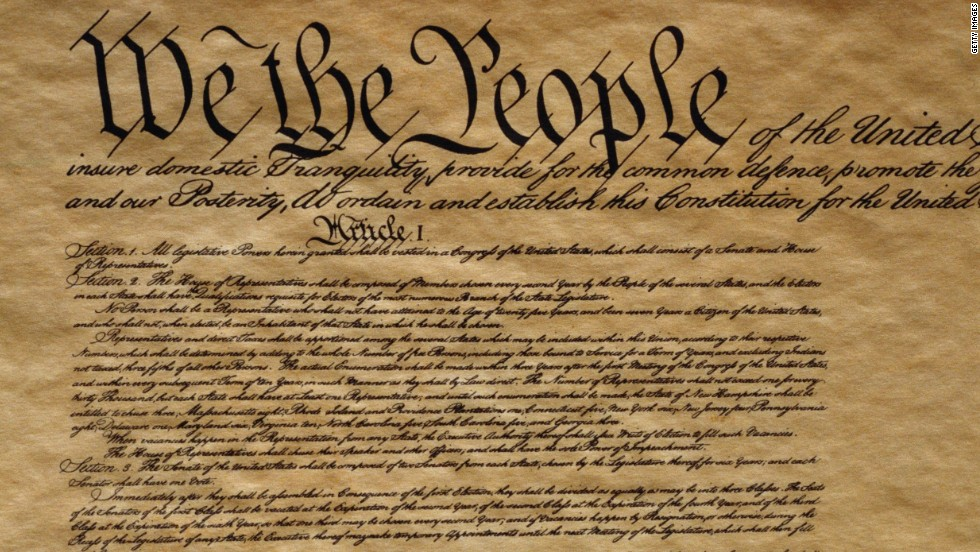
\includegraphics[width=1.0\paperwidth]{we_the_people.jpg}}
  \begin{frame}[plain]
  
%\begin{mdframed}[tikzsetting={draw=black,fill=white,fill opacity=0.7,
%               line width=0pt},backgroundcolor=none,leftmargin=0,
%               rightmargin=40,innertopmargin=4pt]
%\Huge Optimal Turbine Inspections
%\end{mdframed}

  \end{frame}
}

%@@@@@@@@@@@@@@@@@@@@@@@@@@@@@@@@@@@@@@@@@@@@@@@@@
\begin{frame}
\frametitle{How should we read the constitution?}

\begin{itemize}
\item As a historical document?
\bigskip
\bigskip
\item As an expression of political philosophy?
\bigskip
\bigskip
\item As a policy document?
\bigskip
\bigskip
\item As a structure for policy making?
\end{itemize}
\end{frame}

%@@@@@@@@@@@@@@@@@@@@@@@@@@@@@@@@@@@@@@@@@@@@@@@@@
\begin{frame}
\frametitle{How should we read the constitution?}

\begin{itemize}
\item As a historical document?
\bigskip
\bigskip
\item As an expression of political philosophy?
\bigskip
\bigskip
\item \textbf{As a policy document?}
\bigskip
\bigskip
\item \textbf{As a structure for policy making?}
\end{itemize}
\end{frame}

%@@@@@@@@@@@@@@@@@@@@@@@@@@@@@@@@@@@@@@@@@@@@@@@@@
\begin{frame}
\frametitle{How should we read the constitution?  As a policy document?}
\begin{center}
\Large We defined policy as a problem solving intent... so if we are to read the constitution as a policy document, \textbf{what problem is it intended to solve}?
\end{center}
\end{frame}

%@@@@@@@@@@@@@@@@@@@@@@@@@@@@@@@@@@@@@@@@@@@@@@@@@
\begin{frame}
\frametitle{Candidate Problem 1:}

\begin{columns}

\begin{column}{0.5\textwidth}
Let's head back to the 17th century - \textbf{Hobbes Leviathan}: 
\bigskip
\begin{itemize}
\item Given human nature, without government the state of nature must be war of all against all;
\bigskip
\item Need a social contract...
\bigskip
\item That leads to a strong central government!
\end{itemize}

\end{column}

\onslide<1->
\begin{column}{0.5\textwidth}  %%<--- here
    \begin{center}
     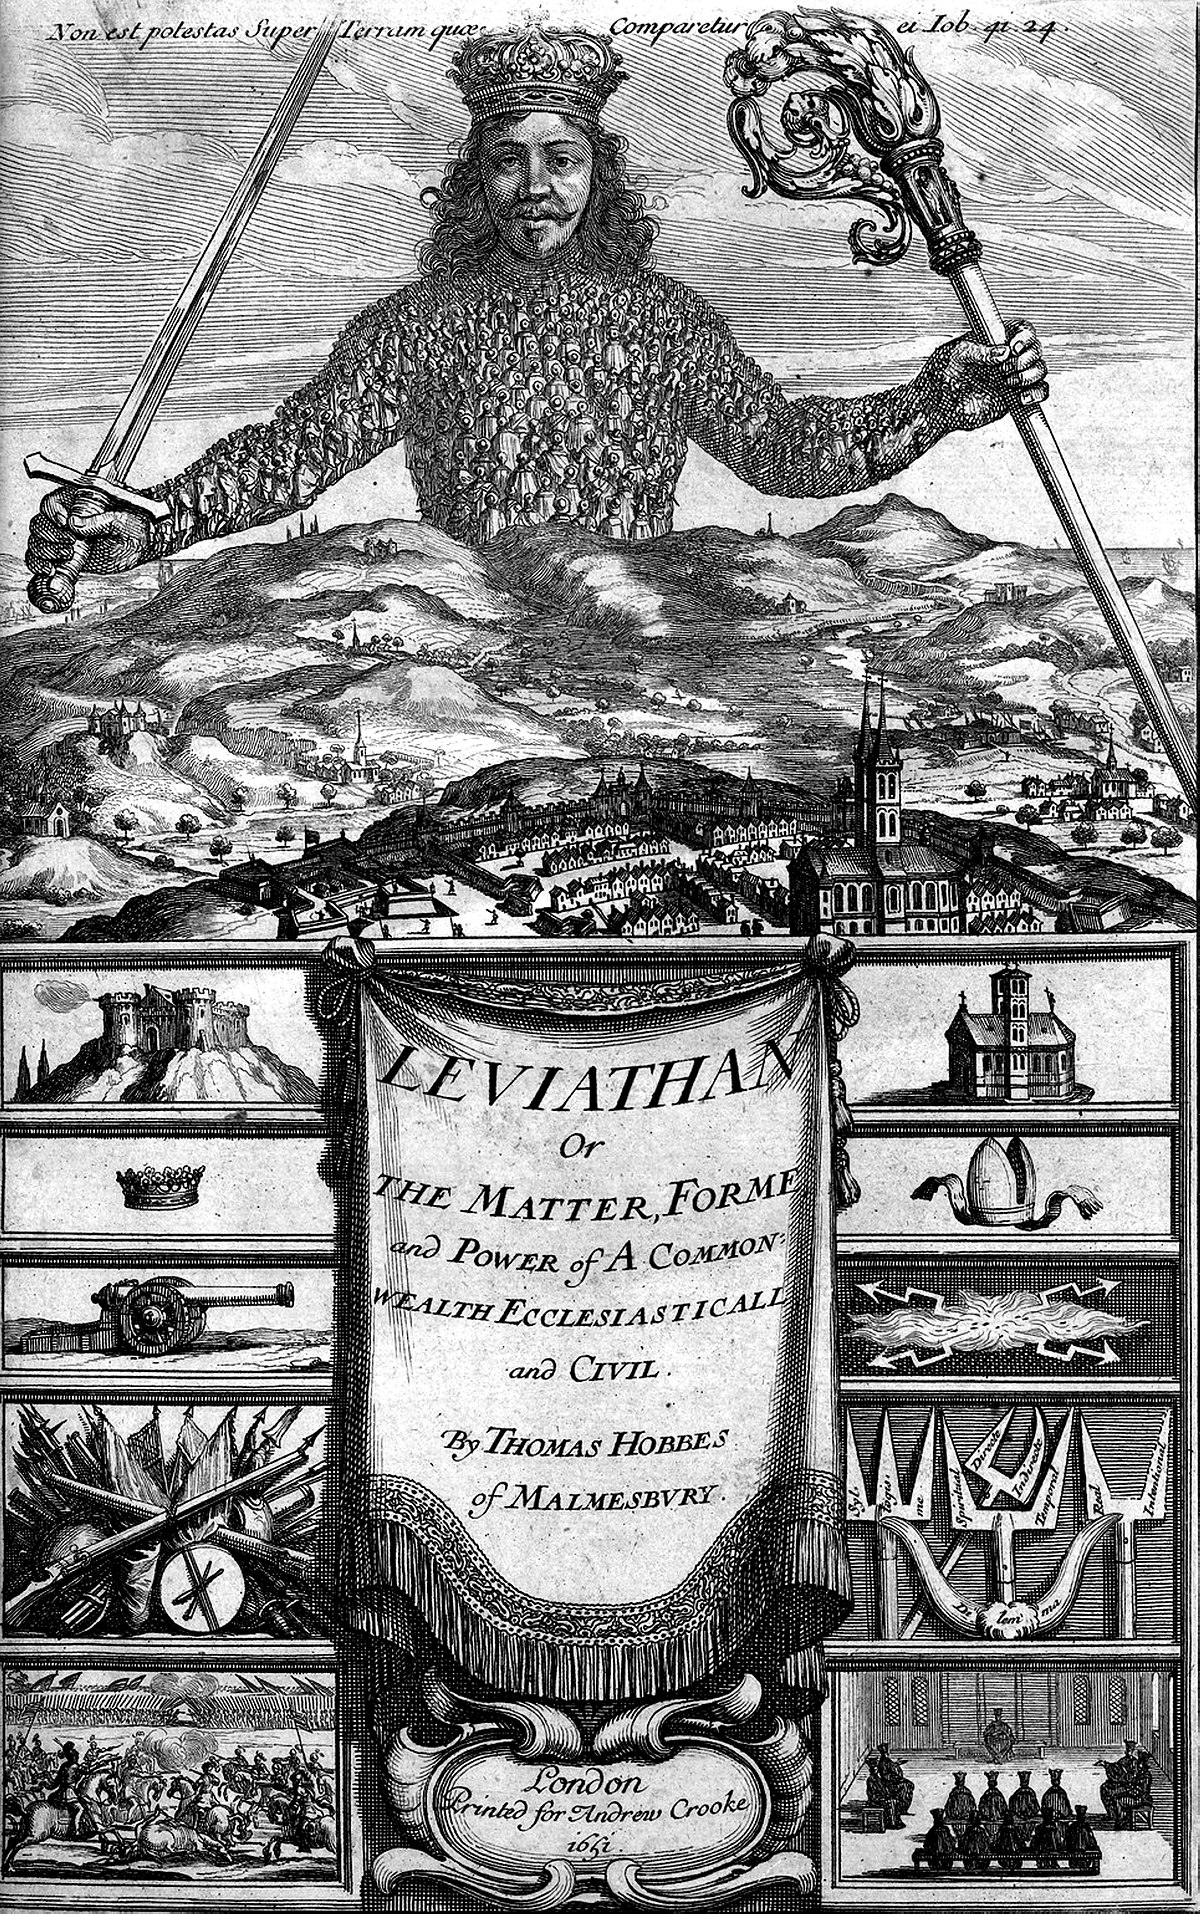
\includegraphics[scale=0.1]{Leviathan.jpg}
     \end{center}
\end{column}

\end{columns}

\end{frame}

%@@@@@@@@@@@@@@@@@@@@@@@@@@@@@@@@@@@@@@@@@@@@@@@@@
\begin{frame}
\frametitle{Candidate Problem 2:}

\begin{columns}

\begin{column}{0.5\textwidth}
Let's head back to the 17th century - \textbf{English Civil War}: 
\bigskip
\begin{itemize}
\item Parliament vs King;
\bigskip
\item How to prevent a tyrannical strong central government?
\end{itemize}
\end{column}

\onslide<1->
\begin{column}{0.5\textwidth}  %%<--- here
    \begin{center}
     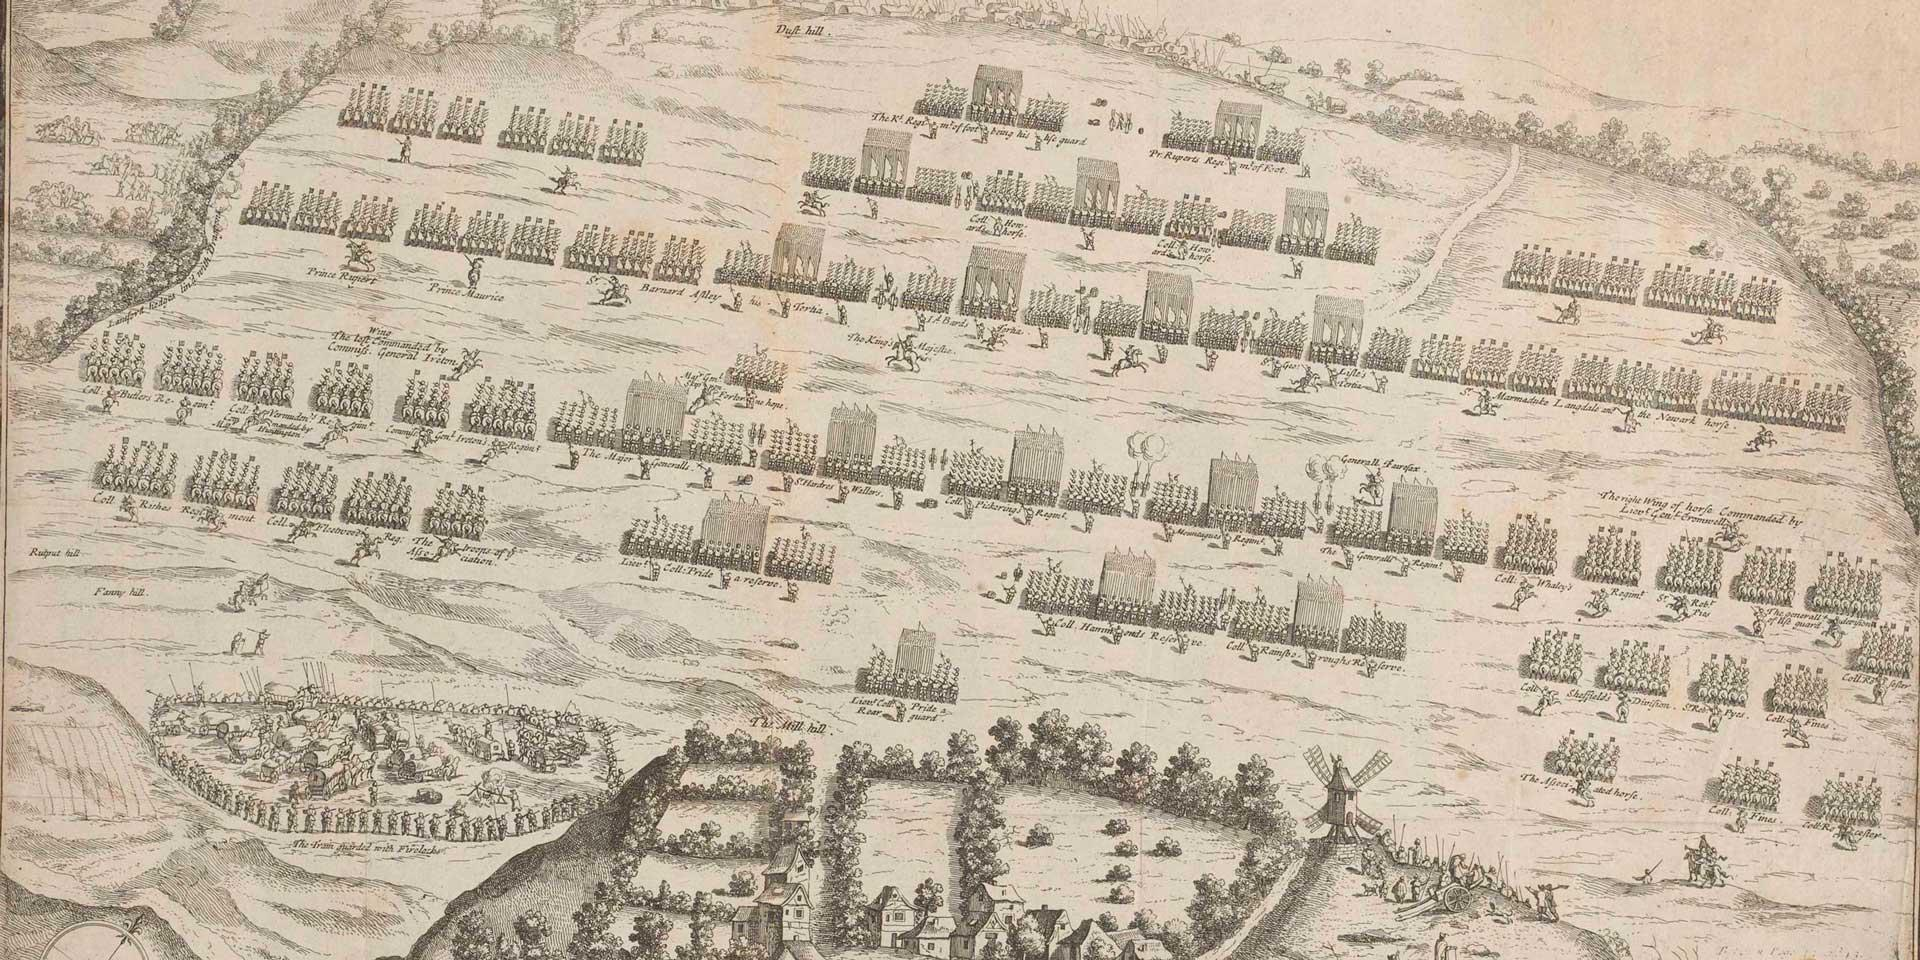
\includegraphics[scale=0.1]{naseby.jpg}
     \end{center}
\end{column}

\end{columns}

\end{frame}

%@@@@@@@@@@@@@@@@@@@@@@@@@@@@@@@@@@@@@@@@@@@@@@@@@
\begin{frame}
\frametitle{How should we read the constitution?  As a structure for policy making?}

The institutional structure of US policy making:
\bigskip
\begin{itemize}
\item affects policy outcomes;
\bigskip
\bigskip
\item is constantly changing.
\end{itemize}

\end{frame}

%@@@@@@@@@@@@@@@@@@@@@@@@@@@@@@@@@@@@@@@@@@@@@@@@@
\begin{frame}
\frametitle{What does the constitution look like?}
\begin{itemize}
\item Article 1: Congress;
\bigskip
\item Article 2: Executive;
\bigskip
\item Article 3: Judiciary;
\bigskip
\item Article 4: relationships between states;
\bigskip
\item Article 5: amendment process;
\bigskip
\item Article 6: supremacy of constitution;
\bigskip
\item Article 7: ratification process.
\end{itemize}

\end{frame}

%@@@@@@@@@@@@@@@@@@@@@@@@@@@@@@@@@@@@@@@@@@@@@@@@@
\begin{frame}

Looking at the setup of each of the first three sections, each tries to answer three questions:
\bigskip
\begin{enumerate}
\item Who are they?
\bigskip
\bigskip
\item How do we get them and get rid of them?
\bigskip
\bigskip
\item What are they allowed to do?
\end{enumerate}

\end{frame}

%@@@@@@@@@@@@@@@@@@@@@@@@@@@@@@@@@@@@@@@@@@@@@@@@@
\begin{frame}
\frametitle{Separation of powers: Article 1, Congress}

\begin{itemize}
\item 1--A Senate and House;
\item 2.3--Representatives and Taxes shall be apportioned, census every 10 years;
\item 2.5--House chooses their Officers and shall have the sole Power of Impeachment;
\item 3.5 \& 3.6--Senate chooses their Officers and shall have the sole Power to try Impeachments;
\item 4.1--States prescribe elections, but Congress may alter such Regulations;
\item 5.2--Two thirds vote to expel a Member;
\item 6--Legislators are paid, privileged from Arrest, may hold no other office;
\item 7--Bills raising revenue start in the House;
\item 7.2 \& 7.3--President's veto can be overruled by two thirds.
\end{itemize}

\end{frame}

%@@@@@@@@@@@@@@@@@@@@@@@@@@@@@@@@@@@@@@@@@@@@@@@@@
\begin{frame}
\frametitle{Separation of powers: Article 1, Congress}

\begin{itemize}
\item 8--Enumerated Powers:
\begin{itemize} 
\item tax and borrow;
\item regulate Commerce;
\item make Rules of Naturalization and Bankruptcy law;
\item coin Money, fix Weights and Measures, punish counterfeiting;
\item establish Post Offices and Roads;
\item promote science and arts through Exclusive Rights to Writings and Discoveries;
\item constitute Tribunals;
\item punish piracies and felonies on the high Seas;
\item declare War;
\item support Armies (for less than two years), maintain a Navy, call the Militia;
\item govern DC and military bases;
\item make all Laws which shall be necessary and proper for carrying into execution the foregoing powers;
\item and all other powers vested by this Constitution in the Government of the United States.
\end{itemize}
\end{itemize}

\end{frame}

%@@@@@@@@@@@@@@@@@@@@@@@@@@@@@@@@@@@@@@@@@@@@@@@@@
\begin{frame}
\frametitle{Separation of powers: Article 1, Congress}

What congress can't do...
\bigskip
\begin{itemize} 
\item 9--Congress may not: suspend Habeas Corpus, issue a bill of attainder, pass ex post facto law, tax exports, grant Titles of Nobility;
\bigskip
\bigskip
\item 9.8--no person holding any office shall accept any present Emolument, Office, or Title, of any kind whatever, from any foreign State;
\end{itemize}
\bigskip
What states can't do...
\begin{itemize}
\item 10--States may not: enter into a treaty, coin Money, pass ex post facto law, grant Titles of Nobility, tax imports or exports (except for inspection), keep troops or engage in War without the Consent of Congress
\end{itemize}

\end{frame}

%@@@@@@@@@@@@@@@@@@@@@@@@@@@@@@@@@@@@@@@@@@@@@@@@@
\begin{frame}
\frametitle{Separation of powers: Article 2, Executive}


\begin{itemize} 
\item 1.1--A president with 4-year terms;
\bigskip

\item 1.2 \& 1.3--Electoral college;
\bigskip

\item 1.7--The President is paid, shall not receive any other Emolument;
\bigskip

\item 2--The President:
\begin{itemize} 
\item shall be CINC;
\item may grant pardons (except in Cases of Impeachment);
\item may make treaties (with consent of two-thirds of the Senate);
\item appoint all Officers of the United States (with consent of the Senate), ``but the Congress may by Law vest the Appointment of such inferior Officers, as they think proper, in the President alone, in the Courts of Law, or in the Heads of Departments";
\end{itemize}
\item 3--Shall give a State of the Union and ``shall take Care that the Laws be faithfully executed";
\bigskip
\item 4--``Shall be removed from Office on Impeachment for, and Conviction of, Treason, Bribery, or other high Crimes and Misdemeanors";
\end{itemize}

\end{frame}

%@@@@@@@@@@@@@@@@@@@@@@@@@@@@@@@@@@@@@@@@@@@@@@@@@
\begin{frame}
\frametitle{Separation of powers: Article 3, Judiciary}

\begin{itemize} 
\item 1--Federal judges serve for life, may not have their pay cut;
\bigskip
\item 2--Cases in Law and Equity, appellate Jurisdiction, "Trial of all Crimes, except in Cases of Impeachment, shall be by Jury";
\bigskip
\begin{itemize}
\item In all Cases affecting Ambassadors, other public Ministers and Consuls, and those in which a State shall be Party, the supreme Court shall have original Jurisdiction;
\bigskip
\item In all the other Cases before mentioned, the Supreme Court shall have appellate Jurisdiction, both as to Law and Fact, with such Exceptions, and under such Regulations as the Congress shall make.- Article III, Section 2;
\bigskip
\end{itemize}
\item 3--Definition of treason: ``Treason against the United States, shall consist only in levying War against them, or in adhering to their Enemies, giving them Aid and Comfort."
\end{itemize}

\end{frame}

%@@@@@@@@@@@@@@@@@@@@@@@@@@@@@@@@@@@@@@@@@@@@@@@@@
\begin{frame}
\frametitle{Division of powers across branches}

\begin{itemize} 
\item Article 1 and Article 2 are rooted in two different kinds of representative democracy.
\bigskip
\bigskip
\item Article 3 is rooted in the idea of wise arbitration, extended to include the authority to restrain the democratic branches through judicial review, where a court strikes laws that it decides are unconstitutional (see Marbury v. Madison). \textbf{Judicial review makes the courts a veto point.}
\end{itemize}

\end{frame}

%@@@@@@@@@@@@@@@@@@@@@@@@@@@@@@@@@@@@@@@@@@@@@@@@@
\begin{frame}
\frametitle{Division of powers across branches}
How do these separated interact across branches?
\bigskip
\begin{itemize} 
\item Presidential veto;
\bigskip
\bigskip
\item Judicial review and deference (e.g. the Chevron doctrine);
\bigskip
\bigskip
\item Legislative delegation.
\end{itemize}

\end{frame}

%@@@@@@@@@@@@@@@@@@@@@@@@@@@@@@@@@@@@@@@@@@@@@@@@@
\begin{frame}
\frametitle{Delegation of powers from branches}


\begin{itemize} 
\item From the legislative branch to the executive branch;
\bigskip
\bigskip
\item From legislative to independent commissions (usually, technically part of the executive, but powers are contested! For example, FERC, FCC, GAO);
\bigskip
\bigskip
\item From higher levels of the executive (president, directors) to lower levels of the bureaucracy;
\bigskip
\bigskip
\item From the federal government (legislative or executive) to states (occasionally also counties, municipalities, nonprofits, companies).
\end{itemize}

\end{frame}

%@@@@@@@@@@@@@@@@@@@@@@@@@@@@@@@@@@@@@@@@@@@@@@@@@
\begin{frame}
\frametitle{Article 4, States' Relations}

\begin{itemize} 
\item 1--Full Faith and Credit shall be given in each state --the courts of one state will enforce laws or judicial decisions of other states;
\bigskip
\item 2.1--Privileges and immunities of individuals... \onslide<2->but NOT corporations: ``A corporation is “the mere creation of local law” and can “have no legal existence beyond the limits of the sovereignty" (Paul v. Virginia)";
\bigskip
\item 2.2--Extradition and Fugitive Slave Clauses: ``No person held to Service or Labour in one State, under the Laws thereof, escaping into another, shall, in Consequence of any Law or Regulation therein, be discharged from such Service or Labour, but shall be delivered up on Claim of the Party to whom such Service or Labour may be due."
\bigskip
\item 2.3--New States may be admitted by Congress
\bigskip

\item 2.4--The United States shall guarantee republicanism, defense against invasion, protection from domestic violence (from Legislature or, if unavailable, the executive); 
\end{itemize}

\end{frame}

%@@@@@@@@@@@@@@@@@@@@@@@@@@@@@@@@@@@@@@@@@@@@@@@@@
\begin{frame}
\frametitle{Article 5, Amendment Process}

\begin{itemize} 
\item The Congress, whenever two-thirds of both Houses shall deem it necessary, shall propose Amendments to this Constitution...
\bigskip
\item ...or, on the Application of the Legislatures of two-thirds of the several States, shall call a Convention for proposing Amendments...
\bigskip
\item ...which, in either Case, shall be valid to all Intents and Purposes, as Part of this Constitution, when ratified by the Legislatures of three-fourths of the several States, or by Conventions in three fourths thereof, as the one or the other Mode of Ratification may be proposed by the Congress...
\bigskip
\item ...Provided that no Amendment which may be made prior to the Year One thousand eight hundred and eight shall in any Manner affect the first and fourth Clauses in the Ninth Section of the first Article; and that no State, without its Consent, shall be deprived of its equal Suffrage in the Senate.
\end{itemize}

\end{frame}

%@@@@@@@@@@@@@@@@@@@@@@@@@@@@@@@@@@@@@@@@@@@@@@@@@
\begin{frame}
\frametitle{Finally, Articles 6 and 7...}

\begin{itemize} 
\item Article 6: Assumption of debts; constitution and following laws are supreme authority; all officials must defend constitution;
\bigskip
\bigskip
\item Article 7: Ratification process.
\end{itemize}

\end{frame}

%@@@@@@@@@@@@@@@@@@@@@@@@@@@@@@@@@@@@@@@@@@@@@@@@@
\begin{frame}
\frametitle{}

\begin{itemize} 
\item Read as a policy document, \textbf{the constitution is a policy for making policies} - it allocates \textbf{authorities} to make, veto, or enforce policy. 
\bigskip
\bigskip
\item The U.S. Constitution and institutions that copy it attempt to separate Legislative, Executive, and Judicial powers, but, in practice, authorities are often unclear or contested.
\bigskip
\bigskip
\item Authorities are reinterpreted to meet the demands of the day.
\end{itemize}

\end{frame}

%@@@@@@@@@@@@@@@@@@@@@@@@@@@@@@@@@@@@@@@@@@@@@@@@@
\begin{frame}
\frametitle{Example: The Commerce Clause}

\begin{itemize} 
\item ``To regulate Commerce with foreign Nations, and among the several States, and with the Indian Tribes;"
\bigskip

\item Wickard v. Filburn, the Supreme Court upheld the New Deal farm subsidies (and corresponding quotas) and crop insurance programs of the Agricultural Adjustment Act;
\bigskip

\item Congress has used commerce clause authority to:
\begin{itemize}
\item Manage food production and other New Deal programs responding to the Great Depression;
\item Prohibit state and businesses from enforcing racial segregation (Civil Rights Act, 1964);
\item Give sexual assault survivors the ability to sue in federal court (Violence Against Women Act, 1994), but the Supreme Court struck this portion of the Act;
\item Incentivize people to have health insurance (ACA, 2010).
\end{itemize}
\end{itemize}

\end{frame}

%@@@@@@@@@@@@@@@@@@@@@@@@@@@@@@@@@@@@@@@@@@@@@@@@@
\begin{frame}
\frametitle{Recapitulation}

\begin{itemize} 
\item Why did we read the Constitution?
\bigskip
\bigskip
\item It is a policy document:
\begin{itemize}
\item ...a proposal for a policy for how to make policies;
\item includes some of the things that such documents need to have;
\end{itemize}
\bigskip
\bigskip
\item It is a structure for making policy:
\begin{itemize}
\item policy making = expression of power;
\item Constitution = power relationships in US political society.
\end{itemize}
\end{itemize}

\end{frame}

%@@@@@@@@@@@@@@@@@@@@@@@@@@@@@@@@@@@@@@@@@@@@@@@@@
\begin{frame}

\begin{center} 
\Huge\textbf{How `good' is the Constitution?}
\end{center}

\end{frame}

%@@@@@@@@@@@@@@@@@@@@@@@@@@@@@@@@@@@@@@@@@@@@@@@@@
\begin{frame}
\frametitle{How `good' is the Constitution?}
\begin{itemize}
\item<1-> Does it have weaknesses?
\bigskip
\bigskip
\item<2-> Are amendments of the original document a sign of strength or weakness?
\bigskip
\bigskip
\item<3-> Does it do enough to create and protect democracy?
\end{itemize}

\end{frame}

%@@@@@@@@@@@@@@@@@@@@@@@@@@@@@@@@@@@@@@@@@@@@@@@@@
\begin{frame}
\frametitle{How `good' is the Constitution?}

\begin{itemize}
\item<1-> How can we judge this?  By introducing the two most important parts of any policy proposal: a \textbf{problem statement} and a set of \textbf{evaluation criteria};
\bigskip
\bigskip

\item<1-> Problem statement = well-defined, scoped statement of the problem to be solved;
\bigskip
\bigskip

\item<2-> Evaluation criteria = a set of standards against which to compare policy proposals:
\bigskip
\begin{center}
\begin{tabular}{ cccc } 
  & Eval Criteria 1 & Eval Criteria 2 & Eval Criteria 3\\ 
 Policy Proposal 1 & No & No & Yes\\ 
 Policy Proposal 2 & Yes & Yes & No \\ 

\end{tabular}
\end{center}
\bigskip
\bigskip
\bigskip
\end{itemize}

\end{frame}

%@@@@@@@@@@@@@@@@@@@@@@@@@@@@@@@@@@@@@@@@@@@@@@@@@
\begin{frame}
\frametitle{How `good' is the Constitution?}

\begin{itemize}
\item<1-> How can we judge this?  By introducing the two most important parts of any policy proposal: a \textbf{problem statement} and a set of \textbf{evaluation criteria};
\bigskip
\bigskip

\item Problem statement = well-defined, scoped statement of the problem to be solved;
\bigskip
\bigskip

\item Evaluation criteria = a set of standards against which to compare policy proposals:
\bigskip
\begin{center}
\begin{tabular}{ cccc } 
  & Minimize time & Avoid Rain & Fight climate change\\ 
Walk & No & No & Yes\\ 
Drive & Yes & Yes & No \\ 

\end{tabular}
\end{center}
\bigskip
\bigskip
\bigskip
\end{itemize}

\end{frame}

%@@@@@@@@@@@@@@@@@@@@@@@@@@@@@@@@@@@@@@@@@@@@@@@@@
\begin{frame}
\frametitle{How `good' is the Constitution?}

Problem statement:\\
\begin{itemize}
\item Create a working government threading the anarchy/tyranny needle;
\item Create a bargain that binds 13 political entities on divergent courses together;
\end{itemize}
\bigskip


\onslide<2->Evaluation criteria:\\
\bigskip
\begin{quote}We the People of the United States, in Order to form a more perfect Union, establish Justice, insure domestic Tranquility, provide for the common defence, promote the general Welfare, and secure the Blessings of Liberty to ourselves and our Posterity...
\end{quote}

\end{frame}

%@@@@@@@@@@@@@@@@@@@@@@@@@@@@@@@@@@@@@@@@@@@@@@@@@
\begin{frame}
\frametitle{How `good' is the Constitution?}

\begin{center}
\Huge\textbf{Does it do enough to create and protect democracy?}
\end{center}

\end{frame}

%@@@@@@@@@@@@@@@@@@@@@@@@@@@@@@@@@@@@@@@@@@@@@@@@@
\begin{frame}
\frametitle{The Election That Could Break America -- Timelines:}

\begin{itemize}
\item<1-> November 3: election day;
\bigskip
\item<2-> December 8: safe harbor deadline for appointing electors;
\bigskip
\item<3-> December 14: electors meet and vote - governors/state Secretaries of State certify elector votes;
\bigskip
\item<4-> January 3: New congress is seated;
\bigskip
\item<5-> January 6: House and senate count and certify votes;
\bigskip
\item<6-> January 20: The incumbent president’s term expires.
\end{itemize}

\end{frame}

%@@@@@@@@@@@@@@@@@@@@@@@@@@@@@@@@@@@@@@@@@@@@@@@@@
\begin{frame}
\frametitle{The Election That Could Break America -- Nightmare scenario: deadlock!}

\begin{itemize}
\item<1-> A state sends two slates of electors to congress and these electors are decisive;
\bigskip
\item<2-> Electoral Count Act ambiguities $\Rightarrow$ VP exercises their certification role and throws out both slates of electors;
\bigskip
\item<3-> Ambiguity in ‘the whole number of voters’ $\Rightarrow$ no majority of electors;
\bigskip
\item<4-> ...$\Rightarrow$ election goes to states with one state one vote;
\bigskip
\item<5-> Speaker expels senators preventing completion of the certification;
\bigskip
\item<6-> Three people with claims to the presidency on inauguration day and no means to decide.
\end{itemize}

\end{frame}

%@@@@@@@@@@@@@@@@@@@@@@@@@@@@@@@@@@@@@@@@@@@@@@@@@
\begin{frame}
\frametitle{How `good' is the Constitution?}

\begin{itemize}
\item “The constitution does not guarantee a peaceful transition of power; it presupposes it”;
\bigskip
\bigskip
\item Evaluation criteria were:
\begin{itemize}
\item ...form a more perfect Union...
\item ...establish Justice...
\item ...insure domestic Tranquility...
\item ...provide for the common defence... 
\item ...promote the general Welfare... 
\item ...and secure the Blessings of Liberty to ourselves and our Posterity.
\end{itemize}
\bigskip
\bigskip
\item Can we redesign electoral policy to prevent a deadlock?  If so how?
\end{itemize}

\end{frame}



%%@@@@@@@@@@@@@@@@@@@@@@@@@@@@@@@@@@@@@@@@@@@@@@@@@
%\begin{frame}
%\frametitle{Week 2 Discussion}
%
%\begin{itemize} 
%\item Great job!  It was thorough and civil!
%\bigskip
%\item Many topics covered: outdated; rigid; court system bias; 10th amendment; House recording; relative power of branches; amendments vs statutes; gov role in combating misinformation; election day holiday; impeachment; electoral college; relationship between founders and religion; franchise extensions and property requirements; freedom of speech; partisanship in the early republic; congressional authorization for use of military force; 2nd amendment; do the constitutional evolution mechanisms necessarily create a powerful presidency; etc...
%\bigskip
%\item Three things left out: gerrymandering, campaign finance, and the decision rule.
%\end{itemize}
%
%\end{frame}
%
%%@@@@@@@@@@@@@@@@@@@@@@@@@@@@@@@@@@@@@@@@@@@@@@@@@
%\begin{frame}
%\frametitle{Week 2 Discussion}
%
%\begin{itemize} 
%\item Constructive criticism: were these \textbf{opinions} or \textbf{arguments}?
%\bigskip
%\bigskip
%\bigskip
%\item Try specifying evaluation criteria and then showing how your view meets those criteria;
%\bigskip
%\bigskip
%\bigskip
%\item Strike words like ``believe" and ``feel" from your vocabulary when you're writing policy and replace with ``assess" or the like.
%\end{itemize}
%
%\end{frame}
%
%%@@@@@@@@@@@@@@@@@@@@@@@@@@@@@@@@@@@@@@@@@@@@@@@@@
%\begin{frame}
%\frametitle{Week 2 Discussion: Example}
%
%\begin{itemize} 
%\item Federalist Papers No. 68: The Mode of Electing the President (Hamilton)
%\bigskip
%\item \small ``It was desirable that the sense of the people should operate in the choice of the person to whom so important a trust was to be confided."
%\bigskip
%\item ``It was equally desirable that the immediate election should made by men most capable of analyzing the qualities adapted to the station and acting under circumstances favorable to deliberation, and to a judicious combination of all the reasons and inducements which were proper to govern their choice."
%\bigskip
%\item ``It was also particularly desirable to afford as little opportunity as possible to tumult and disorder."
%\bigskip
%\item ``Nothing was more to be desired than that every practicable obstacle should be opposed to cabal, intrigue, and corruption."
%\bigskip
%\item ``Another and no less important desideratum was that the executive should be independent for his continuance in office on all but the people themselves."
%\end{itemize}
%
%\end{frame}


\end{document}








